PUMI provides the $O(1)$ queries of intra- and
inter- part mesh topology information needed by ParMA via a complete and
distributed mesh representation~\cite{ibanez2016pumi,WOLFHPC}.
The distributed mesh is the union of mesh parts.
A mesh part is defined as a collection of mesh faces $M^2$ in 2D, and regions
$M^3$ in 3D, assigned to a processing resource, typically a core or hardware
thread.
Mesh entities are denoted as $M^d_i$, where $d$ specifies the
dimension and $i$ specifies the id or index.
At the shared boundary of two or more parts mesh entities are copied (as shown
for mesh vertex $M^0_0$ and edge $M^1_0$ in Fig.~\ref{fig:distMesh}) and
locally tracked on each part through a remote copy object.
Distributed mesh operations involving a mesh entity on the part
boundary are coordinated through an ownership protocol; depicted by the discs
and bold segments in Fig.~\ref{fig:distMesh}.

Two parts with common boundary mesh entities are neighbors.
Sets of mesh entities sharing common neighboring parts form a partition model
entity~\cite{seol2005fmdb}.
Like mesh entities, we denote the i$^{th}$ partition model entity of dimension $d$
as $P^d_i$.
A mesh entity is classified on the partition model entity of equal or greater
dimension which bounds it.
For example, in Fig.~\ref{fig:distMesh} mesh vertex $M^0_0$ is classified on
the partition model vertex $P^0_0$, mesh edge $M^1_0$ is classified on the
partition model edge $P^1_1$, and mesh face $M^2_0$ is classified on the
partition model face $P^2_2$.
These classifications are respectively noted as $M^{0}_0 \sqsubset
P^{0}_{0}$, $M^{1}_1 \sqsubset P^{1}_{1}$, and $M^{2}_0 \sqsubset P^{2}_{2}$.
Information is exchanged by neighboring parts, typically for synchronizing data
associated with part boundary entities, through non-blocking, collective,
neighborhood communications provided by
PCU~\cite{ibanez2016hybrid,ovcharenko2012neighborhood}.

\begin{figure} \centering
  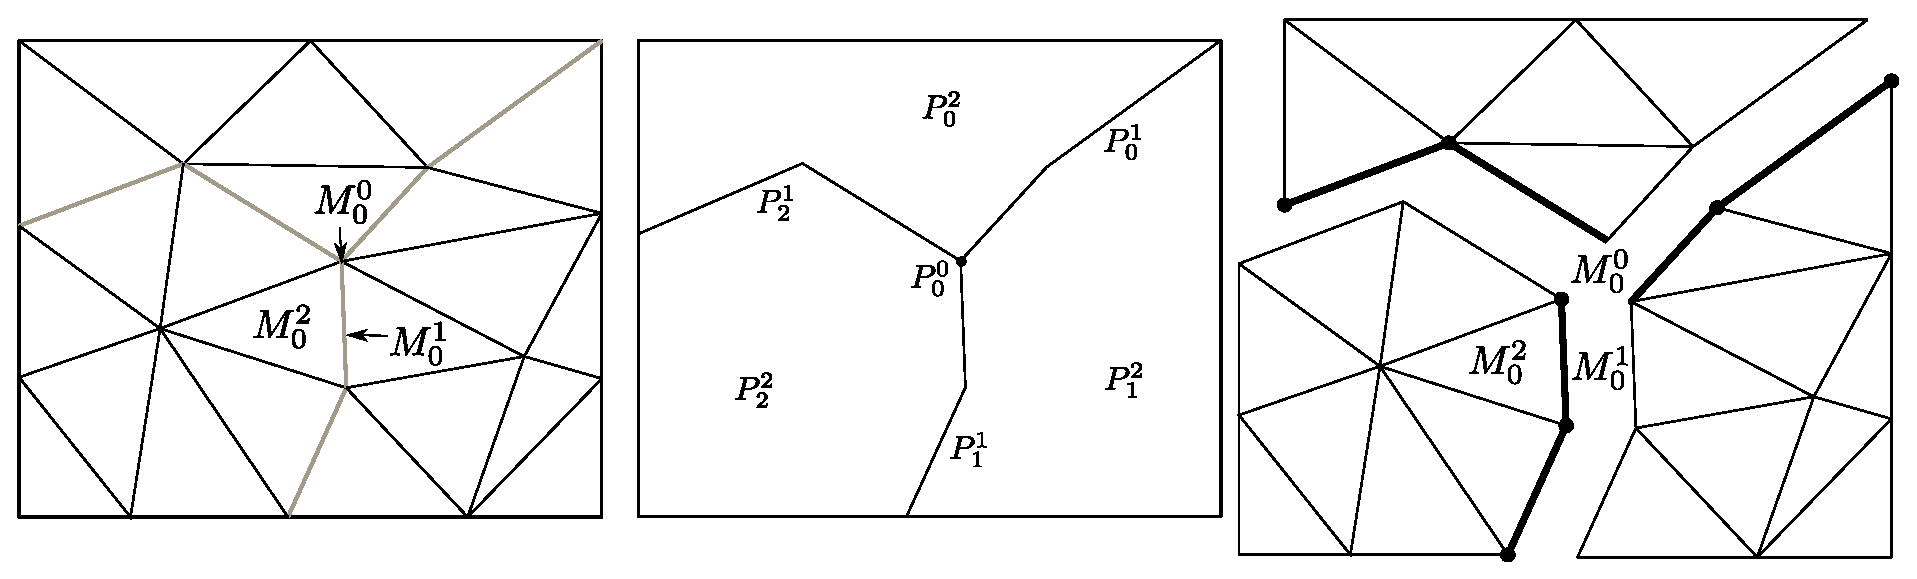
\includegraphics[width=\textwidth]{figs/distMeshAndPtnMdl.eps}
  \caption{
    (left) Example of a mesh, (middle) its partition model, and (right) its
    ownership.
    Discs and bold segments denote entity ownership.
  }
  \label{fig:distMesh}
\end{figure}
